\documentclass[xcolor=table,dvipsnames,svgnames]{beamer}
% Author: alick<alick9188@gmail.com>

% This file is modified from a solution template for:

% - Giving a talk on some subject.
% - The talk is between 15min and 45min long.
% - Style is ornate.

% Copyright 2004 by Till Tantau <tantau@users.sourceforge.net>.
%
% In principle, this file can be redistributed and/or modified under
% the terms of the GNU Public License, version 2.
%
% However, this file is supposed to be a template to be modified
% for your own needs. For this reason, if you use this file as a
% template and not specifically distribute it as part of a another
% package/program, I grant the extra permission to freely copy and
% modify this file as you see fit and even to delete this copyright
% notice.

\mode<presentation>
{
  \usetheme[secheader]{Boadilla}
  \usefonttheme[onlymath]{serif}
  \setbeamercovered{transparent=5}
  \definecolor{thupurple}{HTML}{93278F}
  \definecolor{thudarkpurple}{HTML}{5C307D}
  \definecolor{thulightpurple}{HTML}{BC9BCC}
  \setbeamercolor*{structure}{fg=thupurple}
  \setbeamercolor*{palette primary}{fg=black,bg=thulightpurple}
  \setbeamercolor*{palette secondary}{fg=white,bg=thupurple}
  \setbeamercolor*{palette tertiary}{fg=white,bg=thudarkpurple}
  \setbeamercolor*{palette quaternary}{fg=white,bg=black}
}

\usepackage{graphicx}
\graphicspath{{fig/}}
\usepackage{listings}
\usepackage{xspace}
\usepackage{amsmath}
\usepackage{calligra}
\usepackage{cclicenses} % CC symbols
\usepackage{fontspec}
\usepackage[UTF8,nofonts]{ctex}
\usepackage{hologo}
\usepackage{colortbl}
\usepackage{hyperxmp}
\hypersetup{
pdfauthor={Alick Zhao},
pdfcopyright={Copyright (C) 2015 by Alick Zhao.
Licensed under CC-BY-SA 4.0. Some rights reserved.},
pdflicenseurl={http://creativecommons.org/licenses/by-sa/4.0/},
}

% xeCJK conf setup
\punctstyle{kaiming}
\renewcommand\CJKfamilydefault{\CJKsfdefault} % for slides

\setCJKmainfont[BoldFont={SimHei},
ItalicFont={KaiTi}]{SimSun}
\setCJKsansfont{WenQuanYi Micro Hei}
\setCJKmonofont{WenQuanYi Micro Hei Mono}

\setCJKfamilyfont{zhsong}{SimSun}
\setCJKfamilyfont{zhhei}{SimHei}
\setCJKfamilyfont{zhkai}{KaiTi}

\newcommand*{\songti}{\CJKfamily{zhsong}} % 宋体
\newcommand*{\heiti}{\CJKfamily{zhhei}}   % 黑体
\newcommand*{\kaishu}{\CJKfamily{zhkai}}  % 楷书

\newcommand{\BibTeX}{\hologo{BibTeX}}
\newcommand{\XeTeX}{\hologo{XeTeX}}
\newcommand{\pdfTeX}{\hologo{pdfTeX}}
\newcommand{\beamer}{\textsc{beamer}}
\def\TeXLive{\TeX{} Live\xspace}
\let\TL=\TeXLive
\newcommand{\ThuThesis}{\textsc{ThuThesis}\xspace}

% From thuthesis user guide.
\def\cmd#1{\texttt{\color{DarkBlue}\footnotesize $\backslash$#1}}
\def\env#1{\texttt{\color{DarkBlue}\footnotesize #1}}
\def\cmdxmp#1#2#3{\small{\texttt{\color{DarkBlue}$\backslash$#1}\{#2\}\hspace{1em}\\ $\Rightarrow$\hspace{1em} {#3}\par\vskip1em}}

% For debugging.
%\includeonlyframes{current}

\title
{\ThuThesis 最新动态}

\author[alick] % (optional, use only with lots of authors)
{赵涛\\ \texttt{alick9188@gmail.com}}

\institute[TUNA] % (optional, but mostly needed)
{
  清华大学电子系网络融合实验室
}
% - Use the \inst command only if there are several affiliations.
% - Keep it simple, no one is interested in your street address.

\date
{2015年5月21日}

\subject{ThuThesis, GitHub}

% Delete this, if you do not want the table of contents to pop up at
% the beginning of each subsection:
\AtBeginSubsection[]
{
  \begin{frame}<beamer>{目录}
    \tableofcontents[currentsection,currentsubsection]
  \end{frame}
}


% If you wish to uncover everything in a step-wise fashion, uncomment
% the following command:

%\beamerdefaultoverlayspecification{<+->}

\lstset{basicstyle=\footnotesize\ttfamily,breaklines=true}
\hypersetup{
%pdfpagemode=FullScreen,
}

\logo{
\includegraphics[height=.15\textheight]{tuna-logo.pdf}}

\begin{document}

\begin{frame}
  \titlepage
\end{frame}

\begin{frame}{目录}
  \tableofcontents
  % You might wish to add the option [pausesections]
\end{frame}


% Since this a solution template for a generic talk, very little can
% be said about how it should be structured. However, the talk length
% of between 15min and 45min and the theme suggest that you stick to
% the following rules:

% - Exactly two or three sections (other than the summary).
% - At *most* three subsections per section.
% - Talk about 30s to 2min per frame. So there should be between about
%   15 and 30 frames, all told.

\section{简介}

\begin{frame}{\ThuThesis}
  \framesubtitle{清华大学学位论文 \LaTeX{} 模板}
  \begin{itemize}
  \item 最早:王磊~(2004.4)
  \item 2005 年:薛瑞尼
  \item 最新发布版:\ThuThesis v4.8.1 (2014/12/09)
  \item 全面支持本科、硕士、博士、博士后论文格式
  \end{itemize}
\end{frame}
\section{\ThuThesis 新版本}
\subsection{\ThuThesis 4.8.1}
\subsection{\ThuThesis 4.8.2}
\subsection{\ThuThesis 4.9}
\section{总结}
\begin{frame}{如何使用最新版本?}
      \begin{columns}
        \begin{column}{.7\textwidth}
  \begin{itemize}
    \item 下载最新版
      \begin{itemize}
        \item \url{https://github.com/xueruini/thuthesis}
        \item 右边栏
          \href{https://github.com/xueruini/thuthesis/archive/master.zip}%
          {Download ZIP} 按钮
        %\item Git 用户还可以直接克隆仓库
      \end{itemize}
  \end{itemize}
        \end{column}
        \begin{column}{.3\textwidth}
          \begin{figure}[htbp]
            \centering
            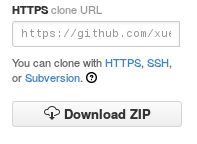
\includegraphics[width=.8\textwidth]{thuthesis-download.png}
          \end{figure}
        \end{column}
      \end{columns}
  \begin{itemize}
    \item 安装
      \begin{itemize}
        \item 解压缩看文档 \texttt{README.md}
        \item 模板文档类:(Xe)LaTeX 引擎处理 \texttt{thuthesis.ins} $\Rightarrow$
          \texttt{thuthesis.cls} 和 \texttt{thuthesis.cfg}
        \item 用户手册:latexmk 处理 \texttt{thuthesis.dtx} $\Rightarrow$
          \texttt{thuthesis.pdf}
        \item 论文示例:latexmk 处理 \texttt{main.tex} $\Rightarrow$
          \texttt{main.pdf}\\
          (或对 \texttt{main.tex} 执行一次 XeLaTeX,一次 BibTeX,再两次
          XeLaTeX)
        \item 可使用或参考附带的 Makefile
      \end{itemize}
  \end{itemize}
\end{frame}

\begin{frame}[fragile]{参考文献}
  \begin{itemize}
    \item 推荐 \BibTeX
      \begin{itemize}
        \item 参考文献管理自动化
        \item bib 文件
        \item bst 参考文献样式文件:\texttt{thubib.bst}
      \end{itemize}
    \item 学校要求两种引用方式:
      \begin{itemize}
        \item 上标模式:如``在许多文献$^{[12,13]}$中……''
        \begin{lstlisting}
  \cite{key12, key13}
        \end{lstlisting}
      \item 正文模式:如``文献~[14] 证明了……''
        \begin{lstlisting}
  \onlinecite{key14}
        \end{lstlisting}
      \end{itemize}
    \end{itemize}
\end{frame}

\section{总结}

\begin{frame}{常见问题}
  \begin{itemize}
  \item \alert{编译不通过} 缺少必要宏包,命令拼写错误,括号未配对等
  \item \alert{表格图片乱跑} \LaTeX{} 自身的浮动定位算法
  \item \alert{段落间距变大} \LaTeX{} 排版算法
  \item \alert{参考文献} 推荐使用 \BibTeX{},也可以手写 \cmd{bibitem}
  \end{itemize}
\end{frame}

\begin{frame}{一点建议}
  \begin{itemize}
    \item 先学习
      \begin{itemize}
        \item 仔细阅读《一份不太简短的~\LaTeXe{} 介绍》(lshort-zh)~(1--2 天)
        \item 粗略阅读《\LaTeXe{} 插图指南》~(2--3 小时)
        \item 仔细阅读《\ThuThesis{} 用户手册》~(20 分钟)
        \item 从~\ThuThesis{} 示例文档入手
      \end{itemize}
  \end{itemize}
\end{frame}

\begin{frame}{利用文档}
  \begin{itemize}
    \item 常用文档
      \begin{itemize}
        \item symbols: 符号大全
        \item Mathmode: 数学参考
        \item ctex, xeCJK: 中文支持
        \item texlive-zh: \TL 安装与使用
        \item 所用宏包文档
      \end{itemize}
    \item 工具
      \begin{itemize}
        \item tlmgr: \TL 管理器
        \item texdoc: \TeX{} 文档查看器\\
          例如:\texttt{texdoc lshort-zh}
      \end{itemize}
  \end{itemize}
\end{frame}

% 寻求帮助
\begin{frame}{求助}
  \begin{columns}[c]
    \begin{column}{.45\textwidth}
      \begin{itemize}
        \item BBS
          \begin{itemize}
            \item \href{http://www.newsmth.net/nForum/board/TeX}{水木
              社区 TeX 版}
            \item \href{http://bbs.ctex.org/}{bbs.ctex.org}
          \end{itemize}
        \item \href{http://www.tex.ac.uk/cgi-bin/texfaq2html}{UK FAQ}
        \item TeX StackExchange
        \item \href{http://justfuckinggoogleit.com/}{Google}
      \end{itemize}
    \end{column}
    \begin{column}{.45\textwidth}
      
\includegraphics[width=\textwidth]{TFZsuperellipse-crop.pdf}
    \end{column}
  \end{columns}
\end{frame}

\begin{frame}{\ThuThesis 问题}
\begin{itemize}
\item GitHub Issues 提问
\item \TeX @newsmth 查找或发文
\item \href{http://groups.google.com/group/thuthesis}\ThuThesis{} Google Group 发问
\end{itemize}
\end{frame}


\begin{frame}{你也可以帮助}
\begin{itemize}
\item 错误反馈:GitHub Issues
\item 改进建议:GitHub Issues
\item 出力维护:LaTeX 宏包编写、Git
\item 科普、答疑\pause \hspace{2em}\alert{图书馆讲座征主讲人!}
\end{itemize}
\end{frame}

\section*{附录}

\begin{frame}
  \begin{itemize}
    \item 本幻灯片:\url{https://github.com/alick/thulib-latex-talk}
    \item 本幻灯片基于:
      \begin{itemize}
        \item \url{http://github.com/alick/fad-texlive-talk}
        \item \ThuThesis{}使用向导 v3.0
      \end{itemize}
    \item 许可证:CC BY-SA 4.0 Unported \cc\ccby\ccsa
  \end{itemize}
\end{frame}

\begin{frame}{扩展阅读}
  \begin{itemize}
    \item \LaTeX\ Tips:
      \url{https://alick.fedorapeople.org/fudcon-apac-2014/latex-tips.pdf} \\
      (例如:\LaTeX{} 中引号的正确输入姿势)
    \item Linux 用户:\url{https://github.com/alick/fad-texlive-talk}
    \item \ThuThesis{}使用向导 v3.0 (薛瑞尼)
    \item \LaTeX{}杂谈(刘海洋)
    \item 《\LaTeX{}入门》(刘海洋)
  \end{itemize}
\end{frame}

\begin{frame}
  \begin{center}
    {\Huge\calligra Thank you!}
  \end{center}
  \begin{figure}[htbp]
    \centering
    %
\includegraphics[height=.2\textheight]{url.pdf}
  \end{figure}
\end{frame}

\end{document}
%%% vim: set sw=2 isk+=\: et tw=80 cc=+1 formatoptions+=mM:
